\documentclass[11pt]{article}
\usepackage{graphicx}
\usepackage{float}
\usepackage{amsmath}
\usepackage{amsfonts}
\usepackage[brazilian]{babel}
\usepackage[utf8]{inputenc}
\usepackage[backend=biber]{biblatex}
\usepackage{csquotes}
\usepackage{gensymb}
%\usepackage{docmute}
\usepackage{array}
\ifdefined\multicol
	\usepackage{multicol}
	\usepackage{geometry}
\fi
\usepackage[T1]{fontenc}
\addbibresource{rel_parcial_erik_perillo_2sem2016.bib}

\newcommand{\fromeng}[1]{\footnote{do inglês: \textit{#1}}}
\newcommand{\tit}[1]{\textit{#1}}
\newcommand{\tbf}[1]{\textbf{#1}}
\newcommand{\ttt}[1]{\texttt{#1}}

\begin{document}

\begin{titlepage}
	\centering
	{\scshape\Large Relatório Parcial\par}
	\vspace{1.5cm}
	{\huge\bfseries Processos atencionais e aprendizado de máquina
		para sistemas robóticos\par}
	\vspace{1cm}
	{\itshape Aluno: Erik de Godoy Perillo\par}
	{\itshape Orientadora: Profa. Dra. Esther Luna Colombini\par}
	\vspace{0.5cm}
	\vfill
    Instituto de Computação\\
	Universidade Estadual de Campinas
	\vfill
	{\large \today\par}
\end{titlepage}

\newpage

\section{Introdução}
A capacidade de percepção e construção de um modelo da realidade ao seu redor
é fundamental para que sistemas robóticos interajam com o ambiente e executem
tarefas diversas e complexas que podem ter as mais variadas utilidades para
os humanos.
Um componente fundamental para isso é a habilidade de dar foco apenas ao
relevante, evitando assim o processamento desnecessário de enormes quantias
de dados.

A atenção é um processo que faz parte do dia a dia de diversos seres vivos
em diversas maneiras e é razoável inspirar-se nela para a construção de
mecanismos semelhantes para a construção de sistemas de inteligência
artificial em máquinas.
Tal área tem sido foco de estudo há anos, resultando em diversas teorias
em psicologia sobre a atenção humana que inspiraram a implementação de
modelos computacionais bem sucedidos.

Neste trabalho, objetivamos construir um modelo atencional eficiente.
Com base no modelo, implementaremos um \tit{framework} atencional para
robôs móveis que permita o uso da seleção em tempo real dos estímulos
mais relevantes para as mais diversas tarefas que o robô possa executar.
No trabalho atual focamos na atenção visual, mas o objetivo
final do sistema é que ele funcione para outros sensores.
O \tit{framework} também contará com um módulo de reconhecimento de objetos
que poderá ser substituído.

\subsection{Objetivos da primeira parte do projeto}
Os objetivos principais para o primeiro semestre do trabalho eram:
\begin{itemize}
    \item Revisão bibliográfica sobre teorias sobre a atenção e diversos
        modelos.
    \item Escolha das técnicas mais adequadas para o processo atencional
        e o reconhecimento de objetos.
    \item Implementação de um modelo atencional.
\end{itemize}
Há uma quantidade surpreendente de avanços recentes na área de modelos
de saliência visual.
Entender os avanços mais relevantes é importante para a obtenção de um sistema
atencional eficiente, então foi requerido mais tempo que o previsto para
essa parte.
Assim, todas as etapas previstas tiveram avanço, com exceção da parte de
reconhecimento de objetos, a qual optamos por deixar para mais tarde pois
a mesma serve como um complemento para nosso trabalho e é de menor relevância
que o componente atencional.
As atividades desenvolvidas são mais detalhadas a seguir.

\section{Resumo das atividades}
\subsection{Revisão Bibliográfica}
Dois dos conceitos importantes para o entendimento da literatura do meio são:
\begin{itemize}
    \item \tit{features}: Características básicas que formam entidades
        visuais, como cor (verde, azul), orientação (horizontal, vertical),
        contraste, tamanho.
    \item \tit{Bottom-up vs. Top-down}: Por componente \tit{bottom-up} de
        atenção entende-se saliências instintivas percebidas por mudanças
        e/ou contrastes muito grandes em uma cena. O componente \tit{top-down}
        é aquele que dá saliência variável às \tit{features} de acordo
        com a meta do agente do momento.
\end{itemize}
A maioria dos modelos computacionais baseia-se em teorias formadas na
psicologia.
Duas das mais famosas são a \tit{Filter Integration Theory} (FIT) e a
\tit{Guided Search}.
Ambas provêm contribuiões importantes para o entendimento dos processos
de saliência visual.
Diversos modelos computacionais foram criados baseando-se em ideias delas.
Começou-se então por elas.

A FIT indica basicamente que se a busca de um objeto de interesse em uma
cena for por apenas uma \tit{feature}, a localização é feita em tempo
instantâneo.
Entretanto, se o objeto de interesse for composto por múltiplas \tit{features}
a serem buscadas (e.g. uma linha horizontal verde),
a localização do objeto é feita em tempo linear.

Já Guided Search diz que buscas por conjunções de \tit{features} são na
verdade mais rápidas pois a combinação das features gera um sinal de
saliência mais forte no campo visual humano.

O VOCUS é um modelo atencional computacional para a detecção de saliências
visuais.
A maioria dos seus componentes é feita com base nas ideias da FIT.
Nesta primeira etapa, exploramos seu componente \tit{bottom-up}.
Ele lida com as \tit{features}: cor, intensidade, orientação.
Seus mapas de saliência são calculados com base nessas \tit{features}
e em diversas dimensões da imagem.

\subsection{Modelo atencional}
A carga teórica adquirida foi útil para a concepção do nosso modelo,
chamado de \tit{att}.
Muitos mecanismos foram inspirados no VOCUS, lidando com as mesmas
\tit{features} e em múltiplas dimensões da imagem.

\subsubsection{Extração de \tit{features}}
O modelo extrai os seguintes mapas de uma certa imagem:
luminância, luminância invertida, vermelho, verde, amarelo, azul,
orientações vertical, horizontal, 45\degree e 135\degree.
Os de luminância e cor podem ser extraídos pela conversão da imagem para o
espaço de cor LAB e as orientações são extraídas usando-se filtros de Gabor.

\subsubsection{Extração de saliência}
Para cada mapa, a saliência é calculada usando-se o mecanismo de
\tit{center-surround}: uma operação que basicamente extrai contrastes fortes
do mapa, dando intensidades de pixel altas para essas regiões.
\begin{figure}[hbt]
\begin{center}
		\begin{tabular} {ccc}
            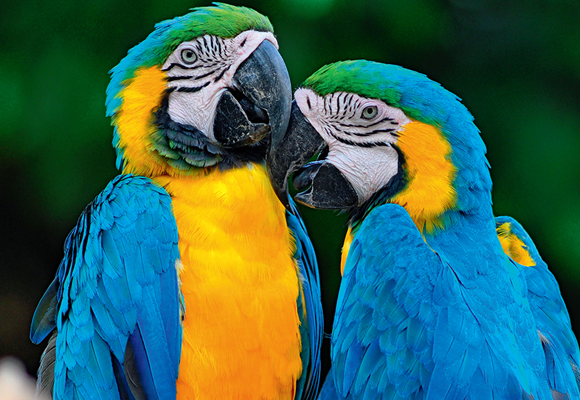
\includegraphics[width=0.3\linewidth]{img/arara.jpg} &
            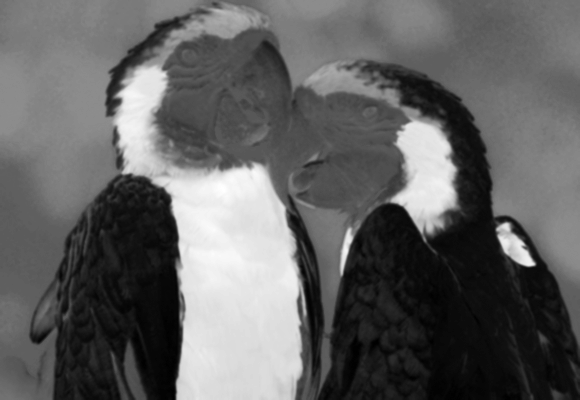
\includegraphics[width=0.3\linewidth]{img/arara_y.png} &
            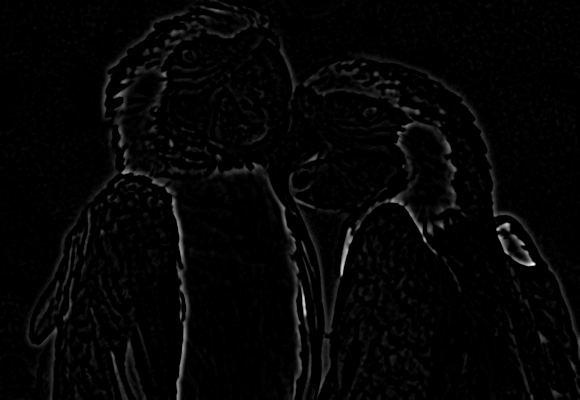
\includegraphics[width=0.3\linewidth]{img/arara_y_cs.png}
		\end{tabular}
\end{center}
\caption{À esquerda, a imagem original. No centro, seu mapa de oponência
amarelo-azul. À direita, o resultado de \tit{center-surround}
no mapa de cor.}
\label{fig:extrfeat}
\end{figure}

\subsubsection{Mapas de saliência para cada instância de \tit{feature}}
Para cada \tit{feature} (e.g\. vermelho) é calculado o
\tit{center-surround}.
Isso é feito na imagem original e em diversas outras dimensões dela,
calculando-se a pirâmide da imagem. Geralmente usamos quatro níveis.
Isso é importante para capturar saliências nos mais diversos níveis de detalhe
da imagem. Uma vez calculados, todos os mapas de uma certa \tit{feature}
são redimensionados para as dimensões originais e somados, formando assim
um mapa de \tit{feature}.

\subsubsection{Normalização}
Uma vez calculados os mapas para cada \tit{feature} (vermelho,
orientação horizontal etc), é preciso fazer uma normalização nos mesmos.
Isso se deve ao fato que, se há grande frequência de picos de saliência
no mapa de vermelho, por exemplo, este não é de muito valor, pois o que se
quer identificar são regiões salientes com relação à imagem como um todo.
Assim, para cada mapa é calculado um peso de normalização.

São diversos os critérios desenvolvidos, como: número de máximos locais,
densidade de máximos locais, espalhamento espacial dos máximos.
Uma análise das alternativas não mostrou muitas diferenças no desempenho,
então opta-se pelo método mais simples, por padrão, que é o número de máximos
locais. Isso pode ser obtido por limiar \tit{Otsu}, seguido de um algoritmo
de componentes conexos para contar os máximos locais.

\subsubsection{Mapas de saliência para cada \tit{feature}}
Uma combinação hierárquica dos mapas é feita após as normalizações.
No final dessa operação, há três mapas: cor, contraste(luminância)
e orientação.
Eles são formados simplesmente somando e normalizando suas instâncias:
O de cor, por exemplo, é formado somando-se os mapas de saliência de
vermelho, verde, amarelo e azul.
\begin{figure}[hbt]
\begin{center}
		\begin{tabular} {ccc}
            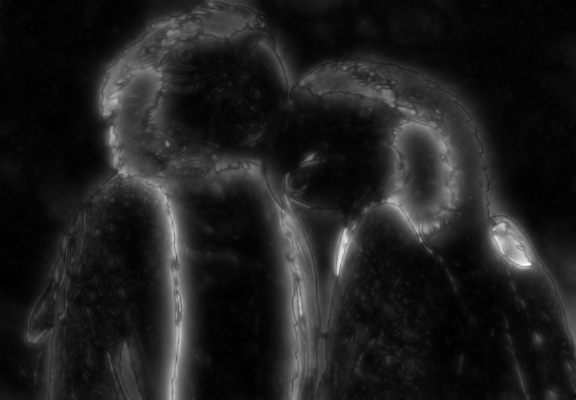
\includegraphics[width=0.3\linewidth]{img/arara_col_map.png}
            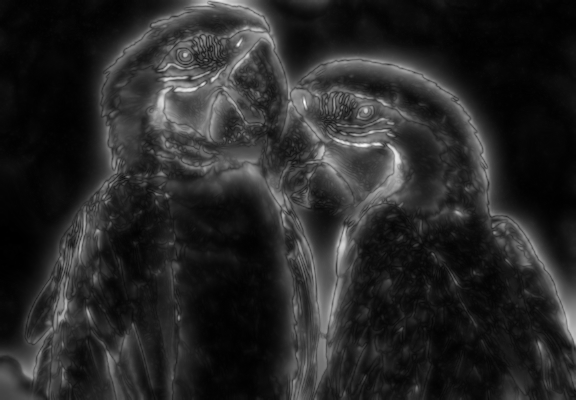
\includegraphics[width=0.3\linewidth]{img/arara_cst_map.png} &
            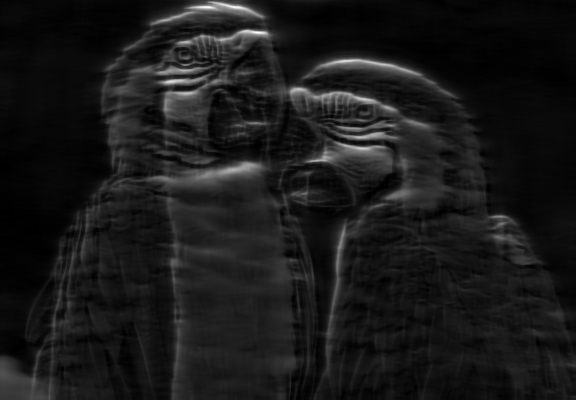
\includegraphics[width=0.3\linewidth]{img/arara_ort_map.png}
		\end{tabular}
\end{center}
\caption{Mapas de saliência da figura original~\ref{fig:extrfeat}.
    Esquerda: mapa de cor. Centro: mapa de contraste. Direita: mapa de
orientação.}
\label{fig:maps}
\end{figure}

\subsubsection{Combinação final}
É dado um peso para cada mapa de saliência (cor, contraste, orientação)
e então eles são somados e normalizados. Nos testes feitos, obteve-se
melhores resultados dando peso maior para a cor e menor para a orientação.
Nos exemplos aqui, os pesos são 2, 1, 0.1 para cor, contraste e orientação,
respectivamente.
\begin{figure}[H]
\begin{center}
        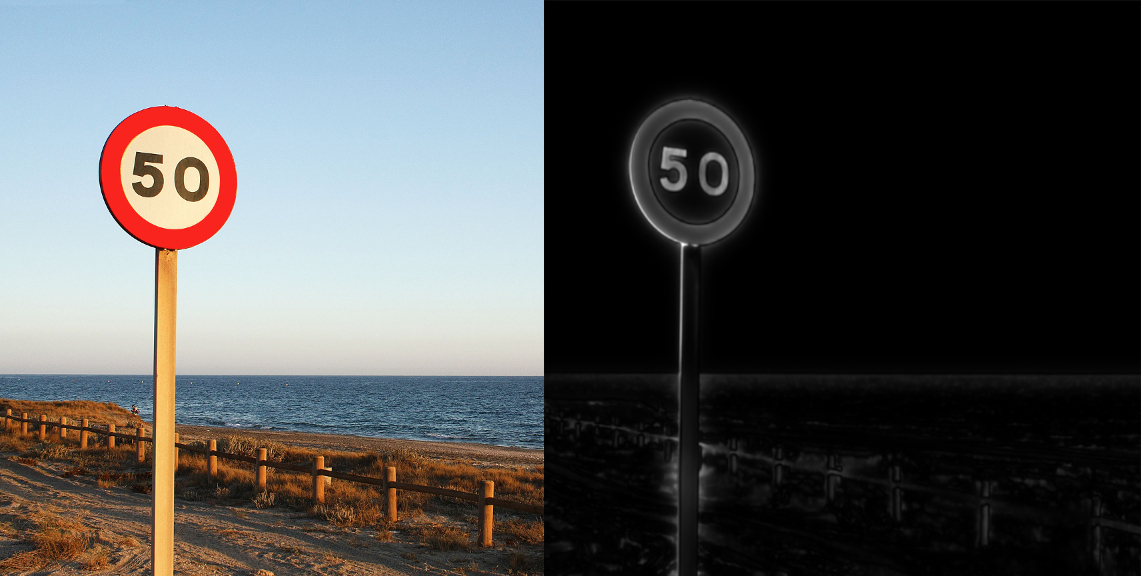
\includegraphics[width=0.6\linewidth]{img/att.png}
\end{center}
\caption{Mapas de saliência final para uma figura. À esquerda, a imagem
original. À direita, o mapa de saliência final.}
\label{fig:att}
\end{figure}

\subsubsection{Implementação}
Todas as etapas do modelo descritas aqui foram implementadas.
A linguagem utilizada foi Python, usando-se OpenCV e numpy.
O código está disponível em (codigo aqui).

\subsubsection{Considerações}
O modelo implementado foi testado em diversas imagens e dá resultados
satisfatórios na maioria dos casos: em regiões intuitivamente mais salientes,
o mapa mostra a região como mais clara (como na figura~\ref{fig:att}).
Há muitos hiperparâmetros para o modelo, como: níveis de pirâmide,
valores dos filtros de Gabor, método de normalização, pesos para os mapas.
Isso exige buscas exaustivas no espaço de alta dimensionalidade dos
hiperparâmetros para achar bons valores, o que é muito custoso.
Assim, embora o modelo atual dê bons resultados, um ponto negativo seu
é a alta quantidade de hiperparâmetros.

\subsubsection{Comparações}
Métricas.
Comparações com modelos no topo.

\subsection{Modelos novos}
Deep learning everywhere.

\section{Produção Científica}
Modelo Att.
Notas: Estudo de métricas.
Estudo de sistemas com Deep Learning.

\section{Próximos passos}
DeepFix. Vídeo.

\printbibliography

\end{document}
